% chap5.tex
%

\mychapter{Human Interaction with Question Answering Systems}
\label{chapter:users}

\noindent

Modern automatic question answering systems are still far from AI machines, that we often imagine or see in the movies.
Many user information needs are still left unanswered by existing automatic question answering systems.
For example, only 36\% of answers of a winning approach from TREC LiveQA 2015 shared task were judged good or excellent.
Therefore, in this chapter I will discuss the research on interactions between a human and a question answering system.

More specifically, Section \ref{sec:user:hints} describes results on studying the effect of hints on user behavior for solving complex informational tasks.
In Section \ref{sec:user:crowd} I propose research on using crowdsourcing for improving the performance of a question answering system.
And Section \ref{sec:user:clarification} shifts the focus towards a dialogue between a user and a QA system, in particular towards clarification questions, that are often needed to understand user's question.

%-=-=-=-=-=-=-=-=-=-=-=-=-=-=-=-=-=-=-=-=-=-=-=-=-=-=-=-=-=-=-=-=-=-=-=-
\section{Search Hints for Complex Informational Tasks}
\label{sec:user:hints}

Search engines are ubiquitous, and millions of people of varying experience use them on daily basis.
Unfortunately, not all searches are successful.
Bilal and Kirby \cite{Bilal:2002:DSI:637512.637516} reported that about half of the participants of their user study felt frustration when searching.
Xie and Cool \cite{xie2009understanding} demonstrated that most of the time users have problems with formulating and refining search queries.
Besides good retrieval performance, a successful search requires users to possess certain skills.
Search skills can be trained, e.g. Google offers a course\footnote{http://www.powersearchingwithgoogle.com} on improving search efficiency.
Although very useful, such courses are time consuming and detached from real search problems of these particular users.
Displaying search hints is another technique that has both learning effect, and offers immediate assistance to the user in solving her current search task.
Moraveji et al. \cite{Moraveji:2011:MIU:2009916.2009966} demonstrated that hints, suggesting certain search engine functionality, help people find answers more quickly, and the effect is retained after a week without hints.

% Besides the awareness about search tools available, adopting general search strategies is extremely important when dealing with a difficult search task.
In my thesis I propose to explore {\em strategic} search hints, that are designed to guide a user in solving her search problem.
More specifically, we chose the divide-and-conquer strategy, \ie splitting an original difficult question into smaller problems, searching answers to the subtasks and combining them together.
Two sets of strategic hints were manually designed: {\em generic} hints describing the divide-and-conquer strategy in general and {\em task-specific} hints providing a concrete strategy to solve the current search task.
To evaluate the effect of the hints on behavior and search success we conducted a user study with 90 participants.
The results of the user study demonstrate that well-designed task-specific hints can improve search success rate.
In contrast, generic search hints, which were too general and harder to follow, had negative effect on user performance and satisfaction.

\subsection{User Study}

\begin{figure}
\centering
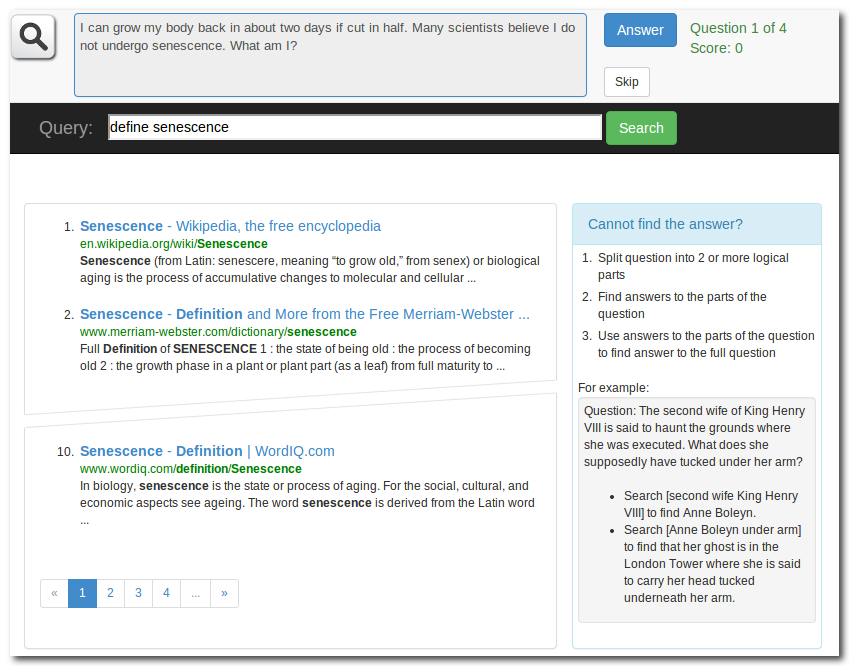
\includegraphics[width=0.75\textwidth]{img/ufindit}
\caption{The interface of the search game used in the study}
\label{figure:ufindit}
\end{figure}

To estimate the effect of strategic search hints on user behavior we conducted a study in a form of a web search game similar to ``a Google a Day''\footnote{http://www.agoogleaday.com/} and uFindIt \cite{Ageev:2011:FYG:2009916.2009965}. Participants were hired using Amazon Mechanical Turk\footnote{http://www.mturk.com/}. 

The goal of the web search game used in the user study is to find answers to several questions with the provided web search interface (Figure \ref{figure:ufindit}). 
Players are instructed not to use any external tools.
% Figure \ref{figure:ufindit} shows the interface of the game.
The questions are given one by one and since tasks might be too difficult, a chance to skip a question was provided, although users were instructed that effort put into solving a question will be evaluated.
To answer a question each player needs to provide a link to a page containing the answer as well as its text.
The answer is automatically verified and a popup box notifies a player if the answer is incorrect (since the answer can be formulated differently, presence of a keyword was checked).
A player can then continue searching or skip the question when she gives up.
A bonus payment was made to players who answer all questions correctly.
We used Bing Search API\footnote{http://www.bing.com/toolbox/bingsearchapi} as a back-end of the game search interface.
All search results and clicked documents were cached so users asking the same query or clicking the same page got the same results.
At the end of the game a questionnaire was presented asking for feedback on user satisfaction with the game, prior experience and other comments.

\begin{table}[tbh]
\centering
\caption{Search tasks used for the study, and specific search hints shown to one of the user groups}
\label{table:tasks}
\begin{tabular}{|p{1cm}|p{4.5cm}|p{4.2cm}|p{6.0cm}|} \hline
 & Question & Correct Answer & Specific hints \\ \hline
Task 1 & I can grow body back in about two days if cut in half. Many scientists think I don't undergo senescence. What am I? & Senescence means ``biological aging''. Hydra is considered biologically immortal and regenerates fast. & \parbox[t]{6cm}{
1. Find what is senescence\\
2. Find who does not undergo senescence\\
3. Find who can also regenerate body and choose the one that satisfies both conditions} \\ \hline
Task 2 & Of the Romans "group of three" gods in the Archaic Triad, which one did not have a Greek counterpart? & Archaic Triad includes Jupiter, Mars and Quirinus. Among those Quirinus didn't have a Greek counterpart. &
\parbox[t]{6cm}{
1. Find the names of the gods from the Archaic triad\\
2. For each of the gods find a Greek counterpart
}\\ \hline
Task 3 & As George surveyed the ``waterless place'', he unearthed some very important eggs of what animal? & "Gobi" in Mongolian means ``Waterless place''. The first whole dinosaur eggs were discovered there in 1923. & \parbox[t]{6cm}{
1. Find what is the ``waterless place'' mentioned in the question?\\
2. Search for important eggs discovery in this ``waterless place''}\\ \hline
Task 4 & If you were in the basin of the Somme River at summers end in 1918, what language would you have had to speak to understand coded British communications? & Cherokee served as code talkers in the Second Battle of the Somme. & \parbox[t]{6cm}{
1. Find the name of the battle mentioned in the questions\\
2. Search for which coded communications language was used in this battle\\
} \\ \hline
\end{tabular}
\end{table}

The tasks for the study were borrowed from the ``A Google a Day'' questions archive.
Such questions are factual, not ambiguous and usually hard to find the answer with a single query, which makes them interesting for user assistance research.
We filtered search results to exclude all pages that discuss solutions to ``A Google a Day'' puzzles.
To do this we removed pages that mention a major part of the search question or ``a google a day'' phrase.
To keep users focused throughout the whole game we limited the number of questions to 4.
The tasks are described in Table \ref{table:tasks} and were presented to all participants in the same order to ensure comparable learning effects.

The questions have multiple parts and to solve them it is helpful to search for answers to parts of the questions and then combine them.
In one of the previous studies we observed, that most of the users didn't adopt the divide-and-conquer strategy, but kept trying to find the ``right'' query.
We decided to estimate the effect of strategic search hints, suggesting users to adopt the new strategy.

We built 2 sets of strategic hints: \textit{task specific} and \textit{generic}.
Task-specific hints described steps of one of the possible solutions to each question (Table \ref{table:tasks}).
Second set contained a single hint, which was shown for all tasks. Generic hint described the divide-and-conquer strategy:\\
\hrule
\begin{enumerate} \itemsep0pt \parskip0pt \parsep0pt
\item Split the question into 2 or more logical parts
\item Find answers to the parts of the question
\item Use answers to the parts of the question to find answer to the full question
\end{enumerate}

For example, the question: ``The second wife of King Henry VIII is said to haunt the grounds where she was executed. What does she supposedly have tucked under her arm?''
\begin{enumerate} \itemsep0pt \parskip0pt \parsep0pt
\item Search [second wife King Henry VIII] to find Anne Boleyn.
\item Search [Anne Boleyn under arm] to find that her ghost is in the London Tower where she is said to carry her head tucked underneath her arm.
\end{enumerate}
\hrule

To control for the learning effect demonstrated in \cite{Moraveji:2011:MIU:2009916.2009966}, each user was assigned to one of the three groups:
\begin{enumerate}\itemsep0pt \parskip0pt \parsep0pt
\item users who didn't get any hints
\item users who got task-specific hints
\item users who got the generic hints
\end{enumerate}


\subsection{Results}

From 199 unique participants, who clicked the HIT on Amazon Mechanical Turk only 90 players finished the game.
We further examined all games manually and filtered out 9 submissions for one of the following reasons: lack of effort (e.g. skipped several tasks after none or a single query) or usage of external resources (e.g. the answer was obtained without submitting any queries or results explored didn't contain the answer).
Furthermore, 10 players from the group which received hints indicated in the survey that they didn't see them, so we filtered out those submissions and finally we had 71 completed games (29 for no hints, 20 for task-specific hints and 22 for generic hints groups).

\subsubsection{Effects of Search Tips on Performance}

In order to measure search success rate we looked at the number of questions answered correctly by different groups of users\footnote{Since users were allowed to skip a question we are counting the number of questions that were eventually solved correctly even if a player made some incorrect attempts}.
Figure \ref{figure:hints:task_success} shows that success rate is higher for users who saw task-specific hints compared to users who didn't get such assistance.
Surprisingly, having the generic hint decreased the success rate, although users could easily ignore a hint they didn't like.
A possible explanation is: generic hints were harder to follow and users who tried and failed became frustrated and didn't restart their searches.

% Similar to \cite{Moraveji:2011:MIU:2009916.2009966} we looked at the average time to answer a question (for this analysis we removed games where a user didn't find the answer and skipped the task).

The plot of average time to answer a question on Figure \ref{figure:hints:task_time} doesn't show an improvement for the task-specific hints group, except for the question 1.
Our task-specific hints represent a possible way to solve a problem and there is no guarantee, that it is the fastest one.
It is worth noting, that users from the generic search hint group had slightly higher variance in success time, which can probably be explained by the fact that some users were successful in finding the right way to follow the hint and some other users struggled with it much longer.
Another insight comes from the number of incorrect attempts users made.
Figure \ref{figure:hints:incorrect} demonstrates the average number of incorrect answer attempts for all groups of users.
Although the variance is high, there is a tendency for users who saw task-specific hints to make less attempts than both other groups.
This is not in direct correspondence with time spent on the game.
It seems that the users who saw a clear strategy to solve the question were less likely to notice plausible, but incorrect solution.
Moreover, we analyzed texts of incorrect answers, and can conclude that a big part of incorrect submission are due to users trying all possible options they found on the way, even if these options are clearly wrong.
% We should note, that unfortunately we didn't limit the number of attempts per problem, thus strategy to verify an answer by submitting it made sense.

\begin{figure}[h]
\centering
  \begin{subfigure}{0.32\textwidth}
  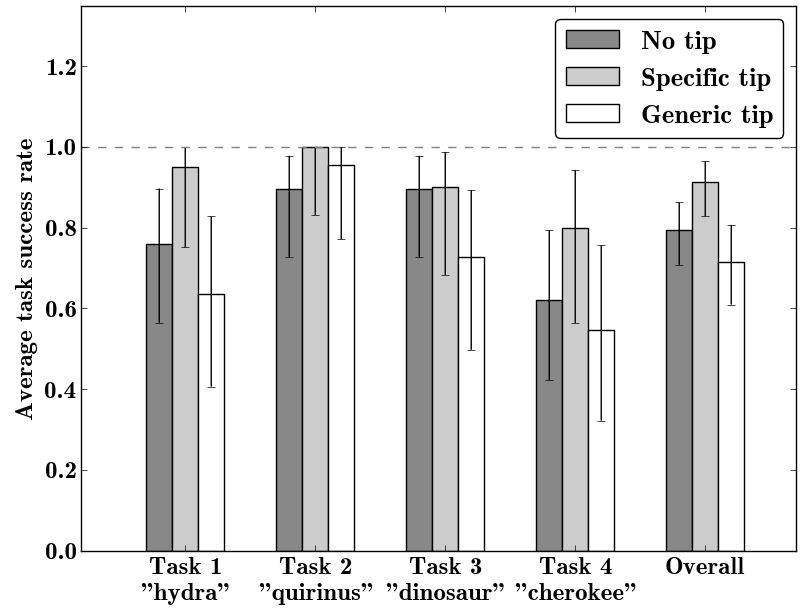
\includegraphics[width=\textwidth]{img/success_per_task}
  \caption{Success rate per task for each group of participants}
  \label{figure:hints:task_success}
  \end{subfigure}
  \begin{subfigure}{0.32\textwidth}
  \centering
  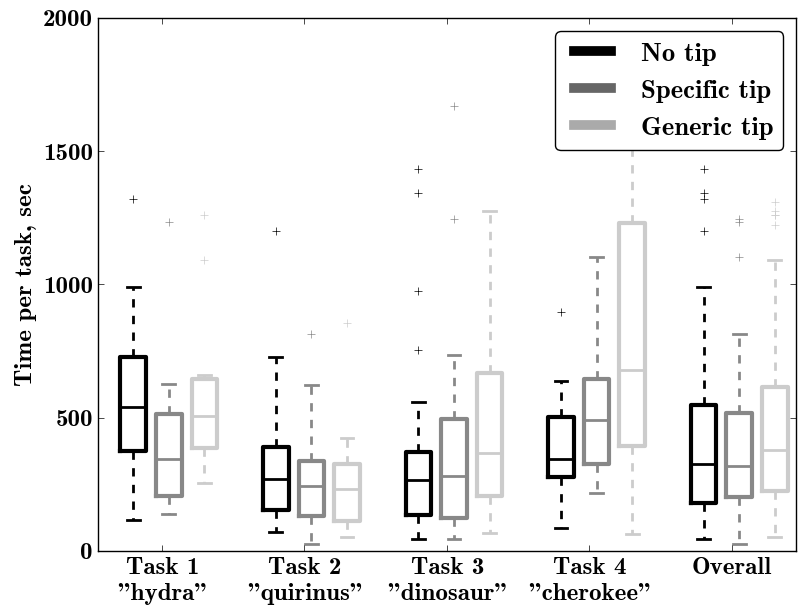
\includegraphics[width=\textwidth]{img/time_per_task}
  \caption{Task completion time for each group of players}
  \label{figure:hints:task_time}
  \end{subfigure}
  \begin{subfigure}{0.32\textwidth}
  \centering
  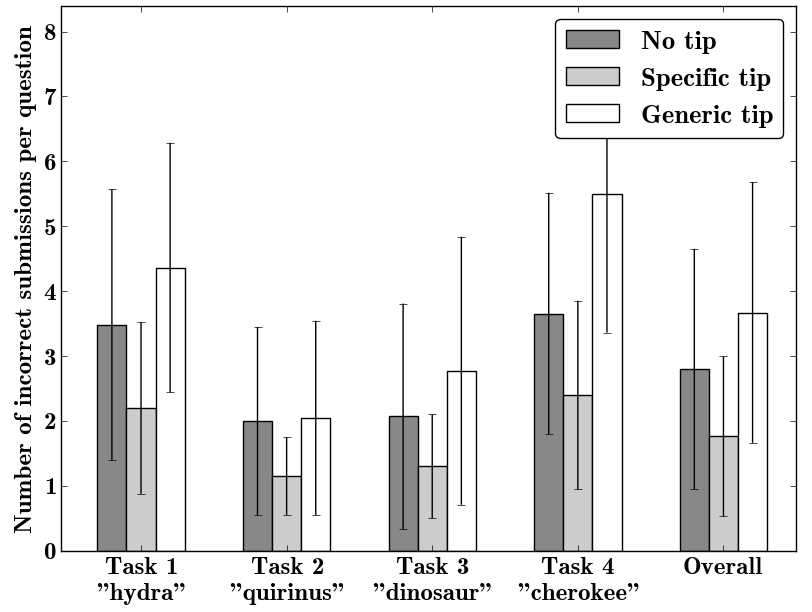
\includegraphics[width=\textwidth]{img/incorrect}
  \caption{The number of incorrect submission attempts per question for all groups of users}
  \label{figure:hints:incorrect}
  \end{subfigure}
\caption{Results of the user study on the effectiveness of strategic search tips on search task success rate}
\label{fig:hints:results}
\end{figure}

\begin{figure}[h]
\centering
\begin{subfigure}[t]{0.32\textwidth}
	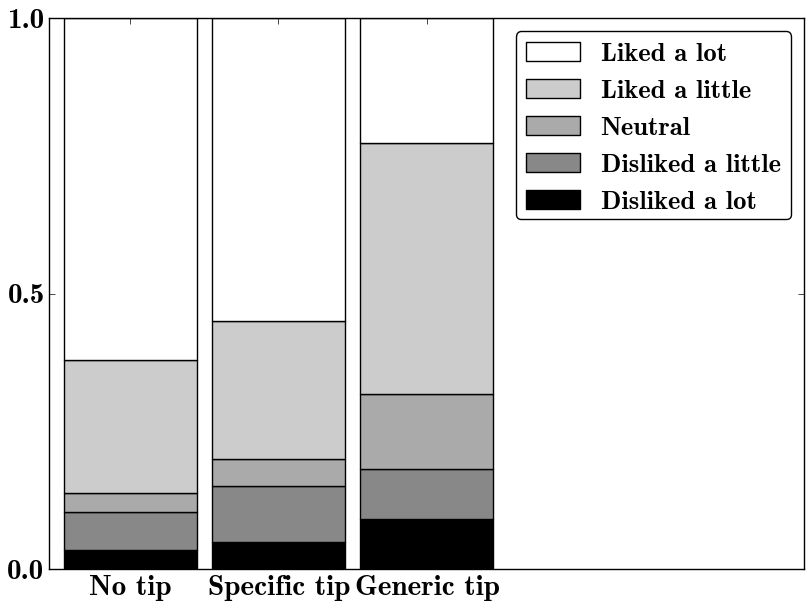
\includegraphics[scale=0.26]{img/liked}
	\caption{How did you like the game?}
    \label{figure:survey:liked}
\end{subfigure}
\begin{subfigure}[t]{0.32\textwidth}
	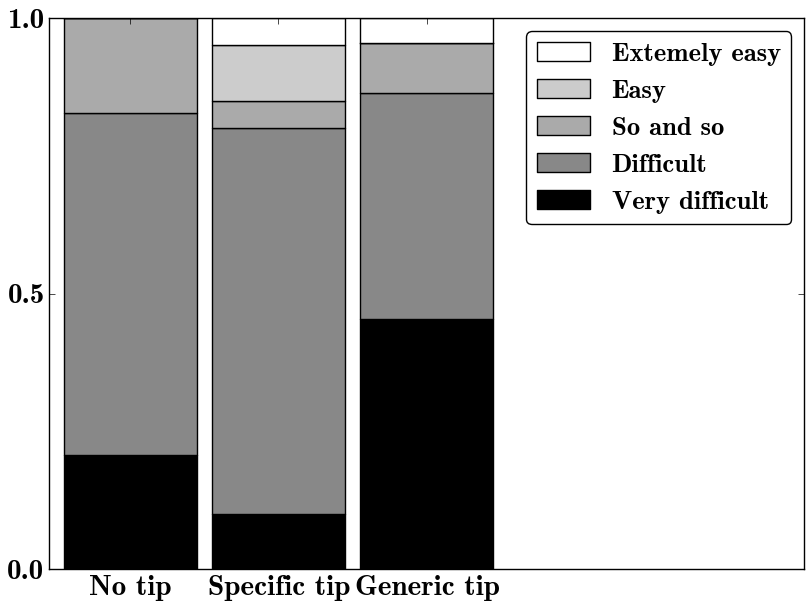
\includegraphics[scale=0.26]{img/difficult}
	\caption{How difficult was the game?}
    \label{figure:survey:difficult}
\end{subfigure}
\begin{subfigure}[t]{0.32\textwidth}
	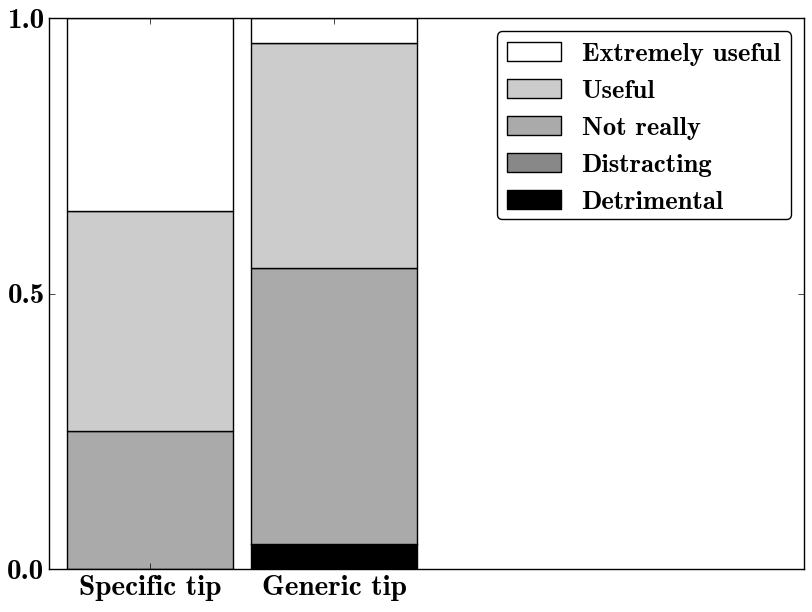
\includegraphics[scale=0.26]{img/useful}
	\caption{Were search hints useful to you?}
    \label{figure:survey:useful}
\end{subfigure}
\caption{Proportions of replies to some of the survey question for each group of users}
\label{figure:hints:survey}
\end{figure}

We also looked at other search behavior characteristics: number of queries submitted, number of clicks made, average length of the queries. The variance in these characteristics was too high to make any speculations regarding their meaning.

\subsubsection{Effects of Search Tips on User Experience}

Finally, we looked at the surveys filled out by each group of users.
Figure \ref{figure:hints:survey} presents proportions of different answers to three of the questions: ``How did you like the game?'', ``How difficult was the game?'' and ``Were search hints useful to you?''.
Surprisingly, user satisfaction with the game was lower for users who saw hints during the game and users who didn't get any assistance enjoyed it more.
The replies to the question about game difficulty are in agreement with the success rate: users who saw task-specific hints rated difficulty lower than participants who struggled to find the correct answers.
The game was very difficult on average, however, some participants from the group who received task-specific hints surprisingly rated it as very easy, which suggests that our hints do help users.
This is supported by the answers to the last question on whether hints were helpful (Figure \ref{figure:survey:useful}).

To summarize, the results of the conducted user study suggest that specific search hints can be helpful, which is indicated by higher success rate, lower number of incorrect attempts and positive feedback in the end of study survey.
In contrast, generic hints can have negative effect on user experience, which is indicated by lower success rate, increased number of incorrect attempts and higher perceived tasks complexity according to the survey.

\subsection{Summary}
In this section we studied the effect of strategic search hints on user behavior. 
The conducted user study in a form of a web search game demonstrated the potential of good hints in improving search success rate.
However, to be useful, they should be designed carefully.
Search hints that are too general can be detrimental to search success.
We also find that even searchers who are more effective using specific search hints, feel subjectively less satisfied and engaged than the control group, indicating that search assistance has to be specific and timely if it is to improve the searcher experience.

We should note, that specific search hints used in this work were manually generated and an interesting question of future work is how to generate such useful hints automatically.
It should be possible to learn strategies applied by the experienced search users and suggest them to the rest.

%-=-=-=-=-=-=-=-=-=-=-=-=-=-=-=-=-=-=-=-=-=-=-=-=-=-=-=-=-=-=-=-=-=-=-=-
\section{Clarification Questions}
\label{sec:user:clarification}

Today, we are observing a possible shift towards natural language interfaces, which will enable richer interaction between a human and computer, in particular question answering.
Most of the existing systems are one-sided, \ie they operate by returning an answer in a response to a user question.
A richer model will inevitably lead to a dialogue rather than request-response kind of communication.
There are many practical aspects of maintaining a dialogue for question-answering.
For example, many questions that user ask allow multiple interpretations, \eg ``FIND GOOD EXAMPLE''.
In such cases a machine could ask a clarification questions to disambiguate certain aspects of the question and provide her with a reasonable response, instead of returning something non-relevant in the first place and force the user to think why did it happen.

Of course, this task is very challenging, and as a first step I propose to study what kind of clarifications do real people typically ask.

%-=-=-=-=-=-=-=-=-=-=-=-=-=-=-=-=-=-=-=-=-=-=-=-=-=-=-=-=-=-=-=-=-=-=-=-
\section{Summary}

SUMMARIZE THE CHAPTER.